%!TEX root = ../../main.tex

\chapter{Theoretische Grundlagen}
\label{theory}

Dieses Kapitel bildet die Grundlage für die folgenden Vergleiche und Evaluationen von Graph Visualisierungen. Es werden Graphen und Knowledge Graphen genauer erläutert, ein Datenformat zur Speicherung der Daten und zuletzt die verschiedenen Visualisierungsoptionen. 

\section{Graphen und Knowledge Graphen}

Graphen sind eine grundlegende Datenstruktur in der Informatik, die aus Knoten und Kanten besteht und zur Modellierung von Netzwerken verwendet wird. Diese Netzwerke können verschiedenste Formen annehmen, von sozialen Netzwerken über Kommunikationsstrukturen bis hin zu biologischen Netzwerken. Die einfache Darstellung von Beziehungen zwischen Entitäten durch Knoten und Kanten macht Graphen zu einem mächtigen Werkzeug für die Datenanalyse und -visualisierung.

In diesem Kapitel werden zunächst die grundlegenden Merkmale von Graphen erläutert und anschließend die besonderen Eigenschaften von Knowledge Graphen vorgestellt. Dabei wird ein besonderer Fokus auf die Unterschiede zwischen traditionellen Graphen und Knowledge Graphen gelegt sowie auf die verschiedenen Anwendungsbereiche, in denen Knowledge Graphen eine Rolle spielen.

\subsection{Definition und Merkmale von Graphen}

Ein Graph ist eine mathematische Struktur, die aus einer Menge von Knoten (engl. vertices) und einer Menge von Kanten (engl. edges) besteht. Die Kanten haben die Aufgabe, Paare von Knoten zu verbinden. Graphen werden verwendet, um Netzwerke zu modellieren, in denen Objekte und deren Beziehungen zueinander abgebildet werden. Diese Netzwerke können unterschiedlichster Natur sein, wie soziale Netzwerke, Kommunikationsnetzwerke oder biologische Netzwerke. Die grundlegenden Merkmale eines Graphen sind seine Knoten, die Entitäten repräsentieren, und die Kanten, die die Beziehungen zwischen diesen Entitäten darstellen (vgl. \cite{graphIntroduction:Wilson}, S. 1 ff.).

Graphen sind besonders wertvoll in der Datenvisualisierung, da sie es ermöglichen, komplexe Beziehungen und Strukturen auf eine Weise darzustellen, die visuell zugänglich und verständlich ist. In der Visualisierung werden Knoten typischerweise durch Kreise oder Punkte dargestellt, während Kanten als Linien oder Pfeile visualisiert werden, die die Richtung und Stärke der Beziehungen anzeigen. Die räumliche Anordnung der Knoten und Kanten spielt dabei eine entscheidende Rolle, da sie die Lesbarkeit und Interpretierbarkeit des Graphen maßgeblich beeinflusst. Verschiedene Layout-Algorithmen können verwendet werden, um die Knoten so anzuordnen, dass Muster wie Cluster oder Hierarchien besser erkennbar werden (vgl. \cite{graphIntroduction:Wilson}, S. 1 ff.). Die verschiedenen Möglichkeiten zur Darstellung von Graphen werden im Kapitel \ref{theory:vistechniques} noch genauer beschrieben.

\subsection{Unterschied zwischen traditionellen Graphen und Knowledge Graphen}

Während traditionelle Graphen primär auf die Darstellung von Entitäten und ihren direkten Beziehungen fokussiert sind, erweitern Knowledge Graphen dieses Modell, indem sie zusätzliche semantische Schichten und Kontextinformationen integrieren. Knowledge Graphen verbinden Entitäten nicht nur durch einfache Beziehungen, sondern auch durch semantische Bedeutungen, die es ermöglichen, komplexe Zusammenhänge und Abhängigkeiten darzustellen. Ein Knowledge Graph ist somit nicht nur eine Struktur von Knoten und Kanten, sondern ein umfassendes Netzwerk, das Entitäten, deren Beziehungen und die zugrundeliegenden Bedeutungen in einem kontextualisierten Modell vereint (vgl. \cite{knowledgeGraphIntroduction:Chaudhri}, S. 17 f.).

\subsection{Anwendungsbereiche von Knowledge Graphen}

Knowledge Graphen finden in einer Vielzahl von Anwendungsbereichen Einsatz, insbesondere dort, wo es auf die Darstellung und Analyse komplexer Beziehungen ankommt. Ein prominentes Beispiel ist der Einsatz von Knowledge Graphen in Suchmaschinen wie Google, wo sie verwendet werden, um Suchergebnisse durch die Verknüpfung von Entitäten und deren Beziehungen kontextualisiert und präzisiert darzustellen. Auch in Sprachassistenten wie Siri oder Alexa spielen Knowledge Graphen eine wichtige Rolle, indem sie die Verbindungen zwischen Begriffen und Konzepten erkennen und nutzen, um relevante und sinnvolle Antworten zu generieren (vgl. \cite{knowledgeGraphIntroduction:Chaudhri}, S. 18 ff.).

Durch die Visualisierung von Knowledge Graphen werden diese komplexen und vernetzten Datenmengen zugänglicher und verständlicher. Die Visualisierung unterstützt nicht nur die Datenanalyse, sondern erleichtert auch die Kommunikation von Erkenntnissen, indem sie abstrakte Zusammenhänge in eine greifbare Form überführt. Dies macht Knowledge Graphen zu einem unverzichtbaren Werkzeug in vielen modernen datengetriebenen Anwendungen (vgl. \cite{knowledgeGraphIntroduction:Chaudhri}, S. 26).

\section{Visualisierungstools für Knowledge Graphen}

Die Visualisierung von Knowledge Graphen ist entscheidend, um komplexe Beziehungen und Datenstrukturen verständlich darzustellen. Diese Visualisierungen ermöglichen es, die semantischen Verbindungen zwischen Entitäten zu erkennen und tiefere Einblicke in die zugrunde liegenden Daten zu gewinnen. In diesem Kapitel werden die Techniken untersucht, die in den weit verbreiteten Visualisierungstools Gephi und Cytoscape eingesetzt werden. Diese Analyse soll die Grundlage für die spätere Implementierung einer eigenen Software bilden.

\subsection{Herausforderungen bei der Visualisierung von Knowledge Graphen}

Die Visualisierung von Knowledge Graphen bringt spezifische Herausforderungen mit sich, die über die traditionellen Anforderungen an Graphvisualisierungen hinausgehen. Das Paper \citetitle{kgVisualization:Nararatwong} beschreibt verschiedene Herrausforderungen, die entscheidend dafür sind, komplexe Datenmengen in einer Weise zu visualisieren, die sowohl zugänglich als auch verständlich ist. In diesem Abschnitt werden die zentralen Herausforderungen beleuchtet, die es bei der effektiven Visualisierung von Knowledge Graphen zu berücksichtigen gilt.

Eine zentrale Herausforderung ist die Skalierbarkeit, insbesondere in Bezug auf die Performance bei großen Datenmengen. Knowledge Graphen bestehen oft aus einer sehr großen Anzahl von Knoten und Kanten, was die Visualisierung vor erhebliche technische Herausforderungen stellt. Die Visualisierungstools müssen in der Lage sein, diese Datenmengen effizient zu verarbeiten und darzustellen, ohne dass die Systemleistung darunter leidet oder die Benutzererfahrung beeinträchtigt wird (vgl. \cite{kgVisualization:Nararatwong}, S. 175). Ein weiterer wichtiger Aspekt ist die Interaktivität. Benutzer müssen die Möglichkeit haben, die Visualisierung dynamisch zu erkunden, um relevante Informationen herauszufiltern und die Daten aus verschiedenen Perspektiven zu betrachten. Dies erfordert Techniken, die eine reibungslose und intuitive Interaktion mit dem Graphen ermöglichen (vgl. \cite{kgVisualization:Nararatwong}, S. 175). Die Verständlichkeit der Darstellung ist ebenfalls von großer Bedeutung. Sie bezieht sich darauf, wie gut die Visualisierung die strukturellen Verbindungen und Bedeutungen zwischen den Entitäten vermittelt. Eine klare und verständliche Darstellung ist notwendig, damit Benutzer die Beziehungen innerhalb des Knowledge Graphen intuitiv erfassen können (vgl. \cite{kgVisualization:Nararatwong}, S. 175).

Das Paper gibt neben den gerade vorgestellten Herausforderungen außerdem auch konkrete Empfehlungen zur Entwicklung eines Visualisierungstools. Eine der zentralen Empfehlungen des Papers ist, die Benutzeroberfläche so zu gestalten, dass sie speziell auf Nicht-Experten ausgerichtet ist. Die Visualisierung sollte den Benutzern eine intuitive und leicht verständliche Schnittstelle bieten, um komplexe Knowledge Graphen zu analysieren und zu verstehen (vgl. \cite{kgVisualization:Nararatwong}, S. 176). Ein weiterer wichtiger Aspekt ist die Leistungsfähigkeit des Visualizers. Um die Verarbeitung großer Datenmengen zu erleichtern, sollte das Backend-System vom UI getrennt werden. Dies ermöglicht die Verlagerung rechenintensiver Aufgaben auf spezialisierte oder skalierbare Servercluster, was die Reaktionsfähigkeit des Visualizers verbessert und die Benutzerfreundlichkeit erhöht (vgl. \cite{kgVisualization:Nararatwong}, S. 176). Zudem empfiehlt das Paper die Implementierung einer modularen Architektur. Ein Knowledge Graph Visualizer sollte erweiterbar und flexibel sein, um neue Technologien und anwendungsspezifische Anforderungen unterstützen zu können. Dies ist entscheidend, um die Anpassungsfähigkeit des Tools zu gewährleisten und es kontinuierlich weiterentwickeln zu können (vgl. \cite{kgVisualization:Nararatwong}, S. 176).

\subsection{Gephi}

Gephi ist ein Open-Source-Tool, das sich auf die Visualisierung und Analyse von Netzwerken spezialisiert hat. Es ist besonders nützlich für die Verarbeitung und Darstellung großer und komplexer Graphen. Ein wesentlicher Vorteil von Gephi liegt in seiner Fähigkeit, große Mengen an Knoten und Kanten effizient zu verarbeiten und darzustellen (vgl. \cite{gephi:Bastian}, S. 1).

Ein zentrales Feature von Gephi ist das Force-Directed Layout (vgl. \cite{gephi:Bastian}, S. 1). Diese Technik simuliert physikalische Kräfte, bei denen Knoten als geladene Teilchen und Kanten als elastische Federn modelliert werden. Dadurch werden die Knoten so angeordnet, dass verwandte Entitäten näher beieinander liegen, was es ermöglicht, Cluster innerhalb des Netzwerks zu identifizieren und die Struktur des Netzwerks verständlicher darzustellen (vgl. \cite{forceGraph:yWorks}). Force-Directed Layouts werden in Gephi häufig eingesetzt, um komplexe Netzwerke intuitiv zu visualisieren.

Darüber hinaus verfügt Gephi über Techniken für Clustering und Community Ermittlung, die es ermöglichen, Gruppen verwandter Knoten in einem Netzwerk zu identifizieren (vgl. \cite{gephi:Bastian}, S. 1 f.). Diese Funktionen sind besonders nützlich für die Analyse semantischer Beziehungen in großen Netzwerken. Durch die Anwendung von Algorithmen können Benutzer Untergruppen innerhalb des Netzwerks erkennen und analysieren, was eine detailliertere Untersuchung der Netzwerkstruktur ermöglicht (vgl. \cite{clusteringGraph:yWorks}).

Ein weiteres nützliches Feature von Gephi ist die Unterstützung für dynamische Graphvisualisierungen. Diese Funktion ermöglicht es, zeitliche Veränderungen in Netzwerken darzustellen, was besonders hilfreich ist, um Entwicklungen über Zeit zu analysieren (vgl. \cite{gephi:Bastian}, S. 2).

Eine der technischen Stärken von Gephi liegt in seiner Unterstützung für GPU-Rendering, das die Verarbeitungsgeschwindigkeit bei der Visualisierung großer Netzwerke erheblich steigert. Durch die Auslagerung rechenintensiver Aufgaben auf die Grafikkarte wird die CPU entlastet, was eine flüssigere und schnellere Darstellung von Graphen ermöglicht. Zusätzlich ist Gephi für Multitasking ausgelegt, was es ermöglicht, mehrere Prozesse gleichzeitig auszuführen, ohne die Gesamtleistung der Software erheblich zu beeinträchtigen. Diese Funktionen sind besonders vorteilhaft bei der Verarbeitung großer Datenmengen und tragen dazu bei, dass Gephi auch bei komplexen Visualisierungsaufgaben effizient arbeitet (vgl. \cite{gephi:Bastian}, S. 1).

Gephi bietet damit eine robuste Plattform für die Visualisierung und Analyse von Netzwerken, wobei der Fokus auf der effizienten Verarbeitung großer Datenmengen und der Unterstützung interaktiver und dynamischer Visualisierungen liegt.

\subsection{Cytoscape}

Cytoscape ist ein Open-Source-Tool, das ursprünglich für die Visualisierung und Analyse von biomolekularen Netzwerken entwickelt wurde. Heute wird es jedoch in verschiedenen Bereichen zur Visualisierung komplexer Netzwerke verwendet, einschließlich Knowledge Graphen (vgl. \cite{cytoscape:Shannon}, S. 1).

Eine wichtige Visualisierungstechnik, die Cytoscape bietet, ist das hierarchische Layout. Dieses Layout ordnet Knoten in einer hierarchischen Struktur an, wodurch Beziehungen zwischen verschiedenen Ebenen eines Netzwerks verdeutlicht werden können. Diese Methode ist besonders nützlich für Netzwerke, die eine natürliche Hierarchie aufweisen, da sie es ermöglicht, die Struktur des Netzwerks klar und strukturiert darzustellen (vgl. \cite{cytoscape:Shannon}, S. 3).

Cytoscape nutzt Edge-Bundling, um visuelle Unordnung in dichten Netzwerken zu reduzieren. Dabei werden Kanten, die in ähnliche Richtungen verlaufen, gebündelt, was die Darstellung von Verbindungen zwischen Knoten deutlich klarer und übersichtlicher macht (vgl. \cite{cytoscapeLayout:Cytoscape}).

Darüber hinaus ermöglicht Cytoscape, die Layouts basierend auf Knotenattributen individuell anzupassen. Diese Funktion erlaubt es den Nutzern, die Visualisierung gezielt nach den relevanten Merkmalen der Knoten auszurichten. Dies ist besonders hilfreich, wenn spezifische Attribute im Fokus der Analyse stehen, da die Darstellung so optimal auf diese abgestimmt werden kann und eine präzisere Untersuchung der Daten ermöglicht wird (vgl. \cite{cytoscape:Shannon}, S. 3 f.).

Ein weiterer wesentlicher Aspekt von Cytoscape ist seine Erweiterbarkeit. Das Tool unterstützt eine Vielzahl von Plugins, die es ermöglichen, die Funktionalität von Cytoscape zu erweitern und an spezifische Anforderungen anzupassen. Diese Erweiterungsfähigkeit macht Cytoscape zu einem flexiblen Werkzeug, das in vielen verschiedenen Anwendungsbereichen eingesetzt werden kann (vgl. \cite{cytoscape:Shannon}, S. 6).

Insgesamt stellt Cytoscape eine robuste Lösung für die Visualisierung von Netzwerken dar, die besonders durch ihre Flexibilität und Erweiterbarkeit überzeugt. Die unterstützten Visualisierungstechniken wie hierarchische Layouts, Edge-Bundling und attributbasierte Layouts ermöglichen es, komplexe Netzwerke strukturiert und übersichtlich darzustellen, was es zu einem wertvollen Werkzeug in der Netzwerkvisualisierung macht.

\section{Visualisierungstechniken}
\label{theory:vistechniques}

Im vorherigen Kapitel wurden die Visualisierungstools Gephi und Cytoscape detailliert analysiert. Dabei wurden die wichtigsten Funktionen und Techniken hervorgehoben, die es den Tools ermöglichen, komplexe Netzwerke zu visualisieren und Verbindungen zwischen Entitäten verständlich darzustellen. Während diese Tools leistungsstarke Frameworks zur Visualisierung bieten, liegt der Fokus dieses Kapitels auf den spezifischen Visualisierungstechniken, die zur Darstellung von Knowledge Graphen verwendet werden können.

Die Wahl der richtigen Visualisierungstechnik ist entscheidend für die effektive Darstellung und Analyse von Knowledge Graphen. Unterschiedliche Techniken haben ihre eigenen Stärken und Schwächen, die je nach Anwendungsfall variieren. In diesem Kapitel werden die gängigen Diagrammarten und Visualisierungstechniken untersucht, die für Knowledge Graphen relevant sind. Es wird aufgezeigt, wie diese Techniken die Darstellung großer und komplexer Datenmengen beeinflussen und welche Aspekte bei der Auswahl der geeigneten Methode berücksichtigt werden sollten.

\subsection{Diagrammarten}
\label{theory:vistechniques:types}

Die Visualisierung spielt eine zentrale Rolle bei der Analyse von Knowledge Graphen, da sie das Verständnis der komplexen Beziehungen zwischen den Entitäten und der Datenstruktur erheblich erleichtert. In diesem Kapitel werden verschiedene Diagrammtypen vorgestellt, die häufig für die Visualisierung von Knowledge Graphen verwendet werden. Dabei werden die jeweiligen Eigenschaften dieser Diagramme hervorgehoben und ihre Vor- und Nachteile erläutert, um eine fundierte Grundlage für die Wahl der geeigneten Visualisierungsmethode zu bieten.

\subsubsection{Node-Link Diagramme}

Node-Link Diagramme sind die intuitivste Art der Graphdaten-Visualisierung. Sie bieten eine zugängliche und visuell ansprechende Möglichkeit, die Vielschichtigkeit von Netzwerken darzustellen. In diesen Diagrammen werden Entitäten als Knoten abgebildet, die meistens durch Kreise dargestellt werden. Um unterschiedliche Typen von Entitäten oder deren Zustände zu kennzeichnen können allerdings auch andere Formen verwendet werden. Die Beziehungen zwischen diesen Entitäten werden durch Linien oder Pfeile dargestellt, wobei häufig verschiedene Stile oder Farben genutzt werden, um die Beschaffenheit oder Intensität dieser Verbindungen zu illustrieren. Die räumliche Positionierung der Knoten und Verbindungen in Node-Link Diagrammen kann die Lesbarkeit sowie die aus der Visualisierung gewonnenen Einsichten stark beeinflussen. Eine sinnvolle Anordnung der Knoten erlaubt es, die spezifischen Charakteristiken des Netzwerks, wie beispielsweise Cluster zu betonen und diese erkennbar zu machen (vgl. \cite{nodelink:Basics}).

Der größte Vorteil von Node-Link Diagrammen besteht in ihrer Fähigkeit, abstrakte relationale Daten begreifbar zu machen. Sie ermöglichen es dem Betrachter, Muster zu entdecken, Unregelmäßigkeiten zu erkennen und die Struktur des Netzwerks durch visuelle Untersuchung zu begreifen. Das macht sie unverzichtbar für jeden Einsatz, bei dem die Beziehungsdynamiken und die Struktur der Daten von Belang sind. Ein Node-Link Diagramm kann beispielsweise in der Analyse sozialer Netzwerke auf einen Blick die Influencer aufzeigen, indem es die Knoten mit den meisten Verbindungen hervorhebt (vgl. \cite{nodelink:Basics}).

Allerdings nimmt die Effektivität von Node-Link Diagrammen mit der Größe und Komplexität des Graphen ab. In dicht vernetzten oder sehr großen Graphen kann die Übersichtlichkeit schnell abnehmen. Überlappende Verbindungen und Knoten führen oft zu einem Durcheinander, das die Visualisierung unklar und verwirrend macht. Dieses Problem kann durch interaktive Visualisierungstools reduziert werden. Diese Werkzeuge erlauben es Nutzern, den Graphen dynamisch zu vergrößern, zu filtern und zu durchsuchen. Dennoch bleibt die Herausforderung der Verständlichkeit bei großen Graphen bestehen (vgl. \cite{nodelink:DynamicGraph}, S. 3). Dies erfordert eine sorgfältige Planung des Diagrammdesigns und den Einsatz von Vereinfachungstechniken wie kraftbasierte Layouts und Kantenverschmelzung, um die Lesbarkeit zu verbessern.

\subsubsection{Adjazenzmatrizen}

Einen gänzlich anderen Ansatz zur Visualisierung von Graphdaten bilden die Adjazenzmatrizen. Sie bieten eine strukturierte und analytische Perspektive auf die Daten. Adjazenzmatrizen verwenden ein rasterbasiertes Layout und eignen sich daher ausgezeichnet für die Abbildung komplexer und großflächiger Netzwerke. Bei einer Adjazenzmatrix werden die Entitäten des Graphen sowohl auf der horizontalen als auch auf der vertikalen Achse einer quadratischen Matrix aufgeführt. Die Zellen innerhalb der Matrix werden gefüllt, um die Existenz einer Beziehung zwischen den entsprechenden Entitäten zu signalisieren. Diese Herangehensweise verwandelt die Vernetzung des Graphen in ein visuelles Muster aus besetzten und unbesetzten Zellen. Eine besetzte Zelle am Kreuzungspunkt der Zeile ii und Spalte jj signalisiert eine direkte Verbindung von Entität ii zu Entität jj (vgl. \cite{adjacencymatrix:Sauras}). Ein Beispiel für die Darstellung eines Node-Link Diagramms als Adjazenzmatrix Diagramm ist in Abbildung \ref{fig:theory:vistechniques:adjacencymatrix} zu sehen.

\begin{figure}[h]
    \centering
    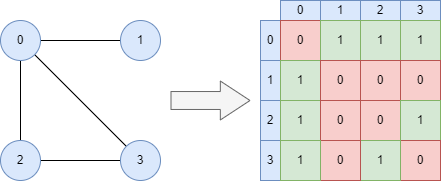
\includegraphics[height=.3\textwidth]{images/02/NodeLinkToAdjacency.drawio.png}
    \caption{Darstellung eines Node-Link Diagramms und dessen Repräsenation als Adjazenzmatrix Diagramm.}
    \label{fig:theory:vistechniques:adjacencymatrix}
\end{figure}

Die Stärke von Adjazenzmatrizen liegt in ihrer kompakten Darstellung großer und dichter Graphen. In solchen Fällen kann ein Node-Link Diagramm, das jeden Knoten und jede Kante visuell darstellt, schnell überladen und unlesbar werden. Im Gegensatz dazu nutzt eine Adjazenzmatrix den Raum optimal. Sie stellt die An- oder Abwesenheit von Kanten zwischen allen Knotenpaaren in einer Rasterstruktur dar. Diese Darstellung hat die Eigenschaft, dass sie keine Überlappungen oder Kreuzungen von Kanten erzeugt, was die Visualisierung deutlich übersichtlicher macht (vgl. \cite{adjacencyOrNode:Okoe}, S. 2941). Da sowohl vorhandene als auch nicht vorhandene Verbindungen in der Matrix dargestellt werden, hängt die Größe der Matrix direkt mit der Anzahl der Knoten zusammen. Das bedeutet, dass unabhängig davon, wie dicht das Netzwerk wird, die Adjazenzmatrix eine konstante Größe beibehält (vgl. \cite{adjacencyOrNode:Okoe}, S. 2945). Diese Eigenschaft macht sie besonders für große Netzwerke geeignet, bei denen ein Node-Link Diagramm zu unübersichtlich wäre.

Die Darstellung der Verbindungen in einer Matrix vereinfacht außerdem das Erkennen von Mustern. Sie ermöglicht eine klare und unmittelbare Visualisierung der Beziehungen zwischen Knoten, wodurch Muster und Cluster leichter erkannt werden können, als dies bei anderen Visualisierungstechniken der Fall ist (vgl. \cite{adjacencyOrNode:Okoe}, S. 2949). Diese Fähigkeit ist in der Datenanalyse besonders wertvoll, da sie eine effiziente und benutzerfreundliche Methode zur Identifizierung von Gruppenstrukturen in komplexen Netzwerken darstellt.

Die Darstellung in Matrixform hilft nicht nur bei der Visualisierung dichter Netzwerke, sondern erhöht auch die Recheneffizienz der Visualisierung. Bei einem Node-Link Diagramm wird viel Rechenleistung benötigt, um die optimale Positionierung der Knoten zu ermitteln. Das Ziel bei der Positionierung der Knoten in Node-Link Diagrammen ist, ein Diagramm zu erzeugen, dass eine hohe Lesbarkeit hat. Um das zu erreichen, wird versucht, ein Layout zu erzeugen, bei dem die Kanten zwischen den Knoten so wenig wie möglich überlappen. Die Berechnung der optimalen Positionierung ist bei großen Netzwerken sehr rechenintensiv. Die Suche nach der optimalen Positionierung entfällt bei Adjazenzmatrizen gänzlich, da die Positionierung durch die Rasterstruktur vorgegeben wird und hier keine Überlappungen entstehen können (vgl. \cite{adjacencyOrNode:Okoe}, S. 2947).

Trotz aller Vorteile von Adjazenzmatrizen gibt es auch einen entscheidenden Nachteil. Adjazenzmatrizen sind für Personen, die nicht mit der Matrixdarstellung von Graphen vertraut sind, weniger zugänglich als Node-Link Diagramme. Das intuitive Verständnis, welches durch die räumliche Anordnung von Knoten und Kanten ermöglicht wird, fehlt hier, was es schwieriger macht, auf den ersten Blick ein intuitives Verständnis für die Gesamtstruktur des Graphen zu entwickeln (vgl. \cite{adjacencyOrNode:Okoe}, S. 2950).

Dennoch bieten Adjazenzmatrizen für bestimmte Aufgaben wie den Vergleich struktureller Ähnlichkeiten zwischen zwei Graphen oder die Durchführung von detaillierten quantitativen Analysen eine unübertroffene Klarheit und Effizienz. Um die Lesbarkeit und analytische Stärke von Adjazenzmatrizen zu verbessern, können verschiedene Techniken angewandt werden, wie etwa das Umordnen der Matrix, um ähnliche Entitäten nebeneinander zu platzieren, oder die Nutzung von Farbverläufen zur Darstellung unterschiedlicher Beziehungsintensitäten. Diese Methoden helfen, die Kluft zwischen struktureller Präsentation und intuitivem Verstehen zu schließen.

\subsubsection{Hierarchische Layouts}

Hierarchische Layouts stellen eine der klassischen Techniken zur Visualisierung von Netzwerken dar, die eine klare Rangordnung oder eine natürliche Hierarchie aufweisen. Diese Layouts ordnen die Knoten eines Graphen in verschiedenen Ebenen an, wobei jede Ebene eine spezifische Hierarchiestufe repräsentiert. Knoten auf derselben Ebene sind in der Regel horizontal oder vertikal ausgerichtet, während die Kanten zwischen den Knoten die Beziehungen zwischen den unterschiedlichen Hierarchiestufen verdeutlichen (vgl. \cite{chen:SurveyGraphVisualization}, S. 630).

Der Hauptvorteil hierarchischer Layouts liegt in ihrer Fähigkeit, die übergeordnete Struktur eines Netzwerks auf eine Weise darzustellen, die für den Benutzer leicht verständlich ist. Diese Layouts ermöglichen es, komplexe Strukturen in einer klaren, baumartigen Darstellung abzubilden, was insbesondere bei der Visualisierung von Organisationen, Entscheidungsprozessen, Klassifikationssystemen oder genealogischen Bäumen von Vorteil ist (vgl. \cite{chen:SurveyGraphVisualization}, S. 629). Durch die visuelle Trennung der Ebenen können Betrachter leicht erkennen, wie sich Informationen oder Autoritäten von einer Hierarchiestufe zur nächsten übertragen.

Ein weiterer Vorteil hierarchischer Layouts ist ihre Effizienz in der Darstellung großer Netzwerke. Indem Knoten in klar definierten Ebenen angeordnet werden, kann visuelles Durcheinander minimiert und eine geordnete Darstellung auch bei umfangreichen Datensätzen gewährleistet werden (vgl. \cite{chen:SurveyGraphVisualization}, S. 630). Dies macht hierarchische Layouts zu einer bevorzugten Wahl für Netzwerke mit zahlreichen Knoten und Kanten, wo andere Visualisierungstechniken möglicherweise an ihre Grenzen stoßen (vgl. \cite{chen:SurveyGraphVisualization}, S. 629).

Trotz ihrer Stärken haben hierarchische Layouts auch einige Einschränkungen. Sie sind weniger geeignet für Netzwerke ohne eine eindeutige Hierarchie oder für solche, bei denen zahlreiche Querverbindungen zwischen den Knoten bestehen (vgl. \cite{chen:SurveyGraphVisualization}, S. 630). In solchen Fällen kann die Darstellung unübersichtlich werden, da die Querverbindungen die klare Struktur des Layouts stören können. Zudem kann es bei sehr komplexen Netzwerken mit vielen Hierarchieebenen schwierig sein, alle Knoten auf begrenztem Raum anzuordnen, ohne dass die Darstellung überladen wirkt.

Ein weiteres Potenzial der hierarchischen Layouts liegt in ihrer Kombination mit interaktiven Visualisierungstechniken. Moderne Tools ermöglichen es dem Benutzer, Teile der Hierarchie einzuklappen oder detaillierter zu untersuchen, was die Benutzerfreundlichkeit und das Verständnis weiter verbessert (vgl. \cite{chen:SurveyGraphVisualization}, S. 631). Dies ist besonders nützlich, wenn nur bestimmte Teile eines Netzwerks für die aktuelle Analyse relevant sind, während andere Bereiche ausgeblendet werden können, um die Übersichtlichkeit zu wahren.

Zusammenfassend bieten hierarchische Layouts eine robuste Methode zur Visualisierung von Netzwerken, die auf Hierarchien beruhen. Sie eignen sich hervorragend für Szenarien, in denen die klare Darstellung von Über- und Unterordnungen im Vordergrund steht und bieten zugleich die Möglichkeit, komplexe Netzwerke in einer geordneten und verständlichen Weise zu präsentieren (vgl. \cite{chen:SurveyGraphVisualization}, S. 630).

\subsection{Vereinfachungs- und Interaktionstechniken}

Im vorherigen Kapitel wurden die verschiedenen Diagrammarten, für die Visualisierung von Knowledge Graphen eingehend beleuchtet. Die Auswahl der richtigen Diagrammart ist entscheidend, um komplexe Zusammenhänge verständlich und übersichtlich darzustellen. Doch selbst mit der optimalen Diagrammart kann die Darstellung umfangreicher Knowledge Graphen schnell an Grenzen stoßen. Vor allem, wenn es darum geht, die Fülle an Informationen für den Betrachter zugänglich zu machen. In diesem Kapitel werden daher Techniken vorgestellt, die eingesetzt werden können, um diese Darstellungen zu vereinfachen und für den Betrachter zugänglicher zu machen.

\subsubsection{Node Clustering}

Eine der effektivsten Methoden zur Vereinfachung komplexer Netzwerke ist das Clustering von Knoten. Beim Node Clustering werden Knoten, die ähnliche Eigenschaften teilen oder eng miteinander verbunden sind, zu sogenannten Clustern zusammengefasst. Diese Technik zielt darauf ab, das visuelle Durcheinander (enlg. visual clutter) eines Graphen zu reduzieren und das Verständnis der Netzwerkstruktur zu erleichtern. Indem verwandte Knoten zu Clustern gruppiert werden, können Benutzer Muster und Beziehungen innerhalb des Netzwerks schneller und klarer erkennen (vgl. \cite{chen:SurveyGraphVisualization}, S. 634).

Die Erkennung von Clustern in Netzwerken stellt jedoch eine signifikante Herausforderung dar, da es keine universelle Definition dafür gibt, was genau einen Cluster ausmacht. Allgemein wird ein Cluster als eine Gruppe von Knoten verstanden, die untereinander stärker verbunden sind als mit Knoten außerhalb des Clusters (vgl. \cite{clustering:AlgosForClust}, S. 1). Die Schwierigkeit besteht jedoch darin, geeignete Kriterien für die Clusterbildung zu definieren und Algorithmen zu wählen, die diese Kriterien in unterschiedlichen Netzwerkstrukturen effektiv umsetzen können. Die Struktur des Netzwerks, die Dichte der Verbindungen und die Art der Daten spielen dabei eine entscheidende Rolle. Ein weiterer komplexer Aspekt ist die Auswahl des richtigen Algorithmus, da verschiedene Methoden unterschiedliche Arten von Clustern erkennen können, was die Vergleichbarkeit der Ergebnisse erschwert.

Eine weit verbreitete Clustering-Methode, die häufig in der Netzwerkvisualisierung angewendet wird, ist der k-Means-Algorithmus. Er hat seinen Namen von der Eigenschaft, dass er die Knoten eines Netzwerks in eine vordefinierte Anzahl von k Clustern einteilt. Der Algorithmus wählt zunächst zufällig k Zentroiden aus, die als Mittelpunkte der Cluster fungieren. Die Knoten werden dann den nächstgelegenen Zentroiden zugewiesen, wodurch vorläufige Cluster entstehen. Der Algorithmus iteriert diesen Prozess, indem er die Position der Zentroiden basierend auf den zugewiesenen Knoten aktualisiert und die Knoten neu gruppiert, bis die Cluster stabil sind und sich die Zuordnungen nicht mehr signifikant ändern (vgl. \cite{kmeans:Xu}, S. 651 f.).

k-Means ist besonders effektiv bei der Aufteilung großer Netzwerke in eine überschaubare Anzahl von Clustern, was die Analyse erleichtert. Ein wesentlicher Vorteil dieses Algorithmus liegt in seiner Einfachheit und seiner Fähigkeit, Netzwerke schnell zu verarbeiten. Allerdings setzt k-Means voraus, dass die Anzahl der Cluster vorab festgelegt wird, was problematisch sein kann, wenn diese Information nicht bekannt ist. Zudem neigt der Algorithmus dazu, Cluster in kugelförmigen Strukturen zu erkennen, was seine Anwendung in Netzwerken mit unregelmäßigen oder komplexen Clusterformen einschränken kann (vgl. \cite{kmeans:Xu}, S. 652 f.).

Der Louvain-Algorithmus ist eine weitere populäre Methode zur Clustererkennung, die speziell für die Analyse großer Netzwerke entwickelt wurde. Im Gegensatz zu k-Means erfordert der Louvain-Algorithmus keine vorherige Festlegung der Anzahl der Cluster. Stattdessen basiert er auf der Optimierung der Modularität, einem Maß, das die Dichte der Verbindungen innerhalb von Clustern im Verhältnis zu den Verbindungen zwischen verschiedenen Clustern beschreibt (vgl. \cite{louvain:Que}, S. 28).

Der Louvain-Algorithmus arbeitet in zwei Hauptphasen. In der ersten Phase werden alle Knoten zunächst als separate Cluster betrachtet. Der Algorithmus iteriert dann über die Knoten und verschiebt jeden Knoten in den Cluster seines Nachbarn, wenn dies die Modularität erhöht. Diese Phase wird wiederholt, bis keine weitere Optimierung der Modularität möglich ist. In der zweiten Phase werden die neu gebildeten Cluster zu Superknoten zusammengefasst, wodurch ein neues Netzwerk auf einer höheren Abstraktionsebene entsteht. Dieser iterative Prozess setzt sich fort, bis die Modularität nicht weiter gesteigert werden kann. Der Louvain-Algorithmus ist besonders effektiv bei der Erkennung von Clustern in Netzwerken, die keine vorab bekannte Struktur aufweisen. Seine Fähigkeit, hierarchische Clusterstrukturen zu erkennen, macht ihn zu einem vielseitigen Werkzeug für die Netzwerkvisualisierung (vgl. \cite{louvain:Que}, S. 28).

\subsubsection{Edge Bundling}

Edge Bundling ist eine Visualisierungstechnik, die entwickelt wurde, um die Darstellung von Netzwerken mit hoher Kantendichte zu vereinfachen. In großen Graphen mit vielen Verbindungen zwischen den Knoten kann es schnell zu einer Überlagerung von Kanten kommen, was die Visualisierung unübersichtlich und schwer interpretierbar macht. Edge Bundling bietet eine Lösung für dieses Problem, indem es Kanten, die ähnliche Verläufe haben, in einem Bündel zusammenführt. Dadurch entsteht eine geordnete Struktur, die es ermöglicht, die wesentlichen Verbindungen innerhalb des Netzwerks leichter zu erkennen (vgl. \cite{edgeBundling:Holten}, S. 1).

Die Technik des Edge Bundling basiert auf der Idee, dass Kanten, die denselben oder einen ähnlichen Verlauf nehmen, in ihrer Darstellung zusammengeführt werden können, ähnlich wie physische Kabel oder Straßen gebündelt werden, um den Verkehr oder Datenfluss effizienter zu organisieren. In der Visualisierung wird dies durch Algorithmen erreicht, die Kanten nach bestimmten Kriterien gruppieren und sie dann gemeinsam in einer visuellen Einheit darstellen. Diese Gruppierung kann auf verschiedenen Attributen basieren, wie z. B. der Nähe der Knoten, den Richtungen der Kanten oder anderen topologischen Merkmalen des Netzwerks (vgl. \cite{edgeBundling:Holten}, S. 2).

Ein bedeutender Vorteil von Edge Bundling ist die erhöhte Lesbarkeit und Verständlichkeit der Netzwerkgrafiken. Durch die Bündelung von Kanten wird die Menge an Informationen, die gleichzeitig dargestellt wird, reduziert, was es den Benutzern erleichtert, Muster und Verbindungen zu identifizieren. Diese Technik ist besonders nützlich, wenn die Analyse des Netzwerks darauf abzielt, übergeordnete Strukturen zu identifizieren (vgl. \cite{edgeBundling:Holten}, S. 2).

Jedoch bringt Edge Bundling auch Herausforderungen mit sich. Ein Nachteil dieser Technik ist, dass einzelne Kanten innerhalb eines Bündels möglicherweise weniger gut sichtbar sind, was zu einem Verlust an Detailgenauigkeit führen kann. Dieser Informationsverlust kann problematisch sein, wenn eine detaillierte Analyse der Verbindungen notwendig ist. Außerdem kann die Wahl der Bündelungskriterien die Interpretation der Daten beeinflussen, da unterschiedliche Algorithmen unterschiedliche visuelle Ergebnisse liefern können (vgl. \cite{edgeBundling:Holten}, S. 2).

\subsubsection{Graph Filterung}

Die Graph Filterung spielt eine entscheidende Rolle sowohl bei der Vorverarbeitung der Daten (engl. preprocessing step), als auch als interaktive Technik in der Visualisierung und Analyse von Knowledge Graphen. Durch die Anwendung von Filtern können irrelevante oder weniger wichtige Knoten und Kanten aus dem Graphen entfernt oder ausgeblendet werden, was die Komplexität reduziert und den Fokus auf relevantere Daten ermöglicht. Dies ist besonders wertvoll bei der Arbeit mit großen Netzwerken, in denen die schiere Menge an Daten die Analyse erschweren kann (vgl. \cite{chen:SurveyGraphVisualization}, S. 634).

Als preprocessing Schritt ermöglicht die Graph Filterung die Reduktion der Datengröße und deren Komplexität, bevor der Graph überhaupt visualisiert wird. In dieser Phase werden Filter angewendet, um nur diejenigen Knoten und Kanten im Graphen zu behalten, die für die spezifische Fragestellung oder Analyse von Bedeutung sind. Durch diese Vorselektion wird sichergestellt, dass die nachfolgende Visualisierung übersichtlicher ist und die Rechenressourcen effizienter genutzt werden. Diese Art der Filterung kann auch dazu beitragen, dass die Visualisierung schneller lädt und reaktionsfähiger ist, da weniger Daten verarbeitet werden müssen (vgl. \cite{chen:SurveyGraphVisualization}, S. 634).

Interaktive Filterung hingegen bietet den Nutzern die Möglichkeit, den Graphen während der Analyse dynamisch zu verändern und anzupassen. Hierbei können Filter in Echtzeit angewendet werden, um bestimmte Knoten und Kanten basierend auf ausgewählten Attributen, wie etwa Verbindungsdichte, Kategorien oder Zeitstempel, ein- oder auszublenden. Diese interaktive Methode erlaubt es den Nutzern, verschiedene Aspekte des Netzwerks zu erkunden und sich auf relevante Teilmengen des Graphen zu konzentrieren.

Durch die Kombination von Filterung beim preprocessing und der interaktiven Filterung können Benutzer den Graphen nicht nur für eine effizientere Verarbeitung vorbereiten, sondern auch während der Analyse flexibel auf die Daten zugreifen und diese an ihre Bedürfnisse anpassen. Diese duale Anwendung der Graph Filterung verbessert die Benutzererfahrung erheblich, indem sie die Komplexität reduziert und gleichzeitig tiefere Einblicke in die Struktur und die Dynamik des Netzwerks ermöglicht.

\subsubsection{Fischaugen-Ansicht}

Die Fischaugen-Ansicht, auch bekannt als Focus+Context oder Fish-eye View, ist eine Interaktionstechnik, die in der Visualisierung komplexer Graphen und Netzwerke verwendet wird. Diese Technik ermöglicht es dem Benutzer, einen bestimmten Bereich des Graphen in einer vergrößerten Darstellung zu betrachten, während der Rest des Netzwerks in einer verkleinerten und weniger detaillierten Ansicht sichtbar bleibt. Das Hauptziel der Fischaugen-Ansicht besteht darin, dem Benutzer eine detaillierte Analyse eines spezifischen Teils des Graphen zu ermöglichen, ohne dabei den Überblick über das gesamte Netzwerk zu verlieren (vgl. \cite{fisheye:Sarkar}, S. 83).

In großen und komplexen Netzwerken kann es schwierig sein, sich auf bestimmte Knoten oder Teilbereiche zu konzentrieren, da die Menge an Informationen und Verbindungen oft überwältigend ist. Die Fischaugen-Ansicht löst dieses Problem, indem sie den Bereich von Interesse vergrößert darstellt und gleichzeitig den Kontext des gesamten Netzwerks beibehält. Dies ermöglicht es dem Benutzer, sowohl die Details des fokussierten Bereichs zu analysieren als auch dessen Position und Beziehung im größeren Netzwerk zu verstehen (vgl. \cite{fisheye:Sarkar}, S. 83).

Technisch gesehen basiert die Fischaugen-Ansicht auf der Idee, die Vergrößerung graduell zu reduzieren, je weiter ein Knoten oder eine Kante vom Fokuspunkt entfernt ist. Im Zentrum des Fokusbereichs wird der Graph stark vergrößert, was eine detaillierte Untersuchung ermöglicht. Je weiter man sich vom Zentrum entfernt, desto stärker wird die Verkleinerung angewendet, bis der Graph schließlich in einer weit entfernten, stark verkleinerten Ansicht dargestellt wird. Diese Technik bietet somit eine verzerrte, aber kontextuelle Darstellung des Netzwerks, die sowohl Detailtreue als auch Übersichtlichkeit vereint (vgl. \cite{fisheye:Sarkar}, S. 83 f.).


Die Fischaugen-Ansicht ist besonders nützlich in Szenarien, in denen Benutzer eine detaillierte Analyse von spezifischen Knoten und deren unmittelbaren Verbindungen vornehmen müssen, während sie gleichzeitig die globalen Muster und Strukturen im Netzwerk im Auge behalten möchten. Ein typisches Anwendungsbeispiel wäre die Untersuchung eines zentralen Knotens in einem sozialen Netzwerk, wo der Benutzer sowohl die direkten Verbindungen dieses Knotens als auch dessen Position und Rolle im gesamten Netzwerk untersuchen möchte. Darüber hinaus kann die Fischaugen-Ansicht auch dynamisch sein, sodass Benutzer interaktiv durch das Netzwerk navigieren können. Der Fokusbereich kann einfach durch Klicken oder Ziehen über den Graphen verschoben werden, wodurch verschiedene Bereiche des Netzwerks schnell und einfach analysiert werden können (vgl. \cite{fisheye:Sarkar}, S. 83 f.).

Zusammenfassend bietet die Fischaugen-Ansicht eine effektive Möglichkeit, in großen und komplexen Netzwerken sowohl den Überblick zu behalten als auch spezifische Details zu untersuchen. Durch die Kombination von fokussierter Vergrößerung und kontextueller Übersicht ermöglicht diese Technik eine tiefere und gleichzeitig umfassende Analyse von Knowledge Graphen, was sie zu einem wertvollen Werkzeug in der Graphvisualisierung macht.